\documentclass[]{article}
\usepackage[utf8]{inputenc}
\usepackage[upright]{fourier}
\usepackage{tikz}
\usetikzlibrary{matrix}
\usepackage{fullpage,amsmath}

\begin{document}
\begin{center}
    \[ H(i,j) = max \left \{
    \begin{array}{lc}
        H(i-1,j-1) + w(a_i,b_j) \quad & \text{Match/Mismatch} \\
        H(i-1,j) + w(a_i,-)     \quad & \text{Deletion}       \\
        H(i,j-1) + w(-,b_j)     \quad & \text{Insertion}      \\
    \end{array} \right\}, 1 \le i \le m, 1 \le j \le n \]

    \[ w(\text{match}) = +2;\quad  w(a,-) = w(-,b) = w(mismatch) = -1 \]

\end{center}

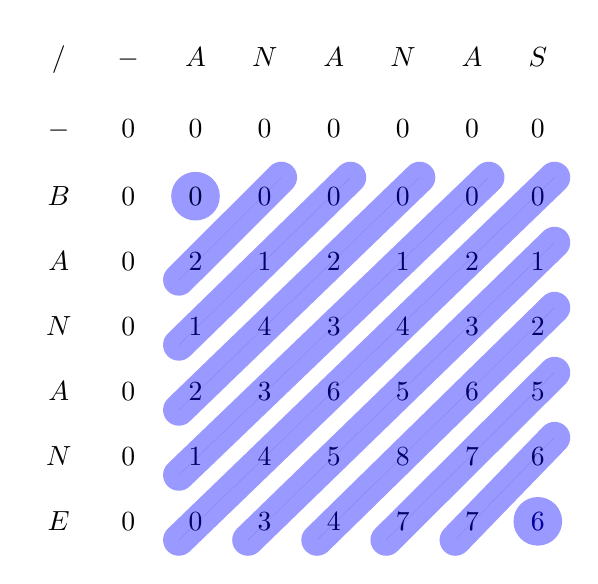
\begin{tikzpicture}[baseline=(sw.center)]
    \tikzset{BarreStyle/.style =   {opacity=.4,line width=4 mm,line cap=round,color=#1}}
    \tikzset{SignePlus/.style =   {opacity=.4,circle,fill=#1}}
    \tikzset{TraceBack/.style =   {opacity=.4,circle,fill=#1}}

    \matrix [%
      matrix of math nodes,
      column sep=1em,
      row sep=1em
    ] (sw) {%
        / & - & A & N & A & N & A & S \\
        - & 0 & 0 & 0 & 0 & 0 & 0 & 0 \\
        B & 0 & 0 & 0 & 0 & 0 & 0 & 0 \\
        A & 0 & 2 & 1 & 2 & 1 & 2 & 1 \\
        N & 0 & 1 & 4 & 3 & 4 & 3 & 2 \\
        A & 0 & 2 & 3 & 6 & 5 & 6 & 5 \\
        N & 0 & 1 & 4 & 5 & 8 & 7 & 6 \\
        E & 0 & 0 & 3 & 4 & 7 & 7 & 6 \\
    };

   % \path
   % (sw-2-3) edge[->] (sw-3-3) (sw-2-4) edge[->] (sw-3-4)
   % (sw-2-5) edge[->] (sw-3-5) (sw-2-6) edge[->] (sw-3-6)
   % (sw-2-7) edge[->] (sw-3-7) (sw-2-8) edge[->] (sw-3-8)

   % (sw-3-2) edge[->] (sw-4-3) (sw-4-3) edge[->] (sw-4-4)
   % (sw-3-4) edge[->] (sw-4-5) (sw-4-5) edge[->] (sw-4-6)
   % (sw-3-6) edge[->] (sw-4-7) (sw-4-7) edge[->] (sw-4-8)

   % (sw-4-3) edge[->] (sw-5-3) (sw-4-3) edge[->] (sw-5-4)
   % (sw-5-4) edge[->] (sw-5-5) (sw-4-5) edge[->] (sw-5-6)
   % (sw-5-6) edge[->] (sw-5-7) (sw-5-7) edge[->] (sw-5-8)

   % (sw-5-2) edge[->] (sw-6-3) (sw-5-4) edge[->] (sw-6-4)
   % (sw-5-4) edge[->] (sw-6-5) (sw-6-5) edge[->] (sw-6-6)
   % (sw-5-6) edge[->] (sw-6-7) (sw-6-7) edge[->] (sw-6-8)

   % (sw-6-2) edge[->] (sw-7-3) (sw-6-4) edge[->] (sw-7-4)
   % (sw-6-5) edge[->] (sw-7-5) (sw-6-5) edge[->] (sw-7-6)
   % (sw-7-6) edge[->] (sw-7-7) (sw-7-7) edge[->] (sw-7-8)

   % (sw-7-3) edge[->] (sw-8-3) (sw-7-4) edge[->] (sw-8-4)
   % (sw-7-5) edge[->] (sw-8-5) (sw-7-6) edge[->] (sw-8-6)
   % (sw-7-6) edge[->] (sw-8-7) (sw-7-7) edge[->] (sw-8-8);

    \draw
    (sw-3-3) node[SignePlus=blue] {$0$}
    [BarreStyle=blue] (sw-4-3.south west) edge[SignePlus=blue] (sw-3-4.north east)
    [BarreStyle=blue] (sw-5-3.south west) edge[SignePlus=blue] (sw-3-5.north east)
    [BarreStyle=blue] (sw-6-3.south west) edge[SignePlus=blue] (sw-3-6.north east)
    [BarreStyle=blue] (sw-7-3.south west) edge[SignePlus=blue] (sw-3-7.north east)
    [BarreStyle=blue] (sw-8-3.south west) edge[SignePlus=blue] (sw-3-8.north east)
    [BarreStyle=blue] (sw-8-4.south west) edge[SignePlus=blue] (sw-4-8.north east)
    [BarreStyle=blue] (sw-8-5.south west) edge[SignePlus=blue] (sw-5-8.north east)
    [BarreStyle=blue] (sw-8-6.south west) edge[SignePlus=blue] (sw-6-8.north east)
    [BarreStyle=blue] (sw-8-7.south west) edge[SignePlus=blue] (sw-7-8.north east)
    (sw-8-8) node[SignePlus=blue] {$6$}
    %(sw-7-6) node[TraceBack=red] {$8$} (sw-6-5) edge[->] (sw-7-6)
    %(sw-6-5) node[TraceBack=red] {$6$} (sw-5-4) edge[->] (sw-6-5)
    %(sw-5-4) node[TraceBack=red] {$4$} (sw-4-3) edge[->] (sw-5-4)
    %(sw-4-3) node[TraceBack=red] {$2$} (sw-3-2) edge[->] (sw-4-3)
    ;
\end{tikzpicture}
\end{document}
